\section{Implementation}\label{sec:trans_implementation}
Armed with the specifications and design decisions mentioned in Section \ref{sec:trans_theory} it is time to step into the implementation phase. In practice this process is iterative, and the demands sometimes change with issues that emerge while working. This section aims to explain this process and describe some of the iterative steps that were taken.


\subsection{General structure}
To first give an overview of how the transport layer protocol is implemented, the general design structure is going to be clarified in the following: When first beginning the process of writing code, two main entities were identified. One is the protocol system itself, and other the packet data structure. These two are implemented as the C++ classes \custtt{DtmfTransport} and \custtt{Packet}.

The \custtt{DtmfTransport} class takes care of the connection and most of the features described in the design specifications. It is both the interface to the rest of the system and also the connection caretaker. With this, I mean that \custtt{DtmfTransport} is essentially initiating, maintaining and closing connections - although it all happens on command of the user (through the API). The \custtt{DtmfTransport} class makes use of the services provided by the \custtt{Packet} class to be able to set up, and manipulate, packet data structures.

\custtt{Packet} directly represents the packet format as it is specified in Section \ref{sub:trans_packet_format}, meaning it basically consists of 8 bytes of header and up to 248 bytes of data. Add to that a number of methods to access or manipulate private members. The most important of these methods is probably \custtt{make()}, which is working as a so-called \textit{lazy constructor}. Constructing lazily means that the \custtt{Packet} data members are not filled in before \custtt{make()} is called. Thus, \custtt{packet} objects can be passed around even without anything ''in them''.


\subsection{Function classification}
To better gain an overview of of which functions are doing what, they are split into two classifications: Essential- and compatibility functions. The essential functions are the ones providing functionality by directly implementing features, as described in the protocol design section. Compatibility functions are functions which are added to make the protocol compatible with other parts of the networking system.

\begin{table}[htb]
 \centering
 \begin{tabular}{lll}
  %      & \multicolumn{2}{c}{l}\\
  Class & Essential & Compatibility \\
  \midrule
  \smalltt{DtmfTransport}  & \smalltt{encode()}          & \smalltt{toPacketQueueFromApi()}  \\
                           & \smalltt{decode()}          & \smalltt{packetFromCharBuffer()}  \\
                           & \smalltt{setPort()}         & \smalltt{packetToCharBuffer()}    \\
                           & \smalltt{connect()}                                             \\
                           & \smalltt{close()}                                               \\
                           & \smalltt{port()}                                               \\
                           & \smalltt{connStatus()}                                           \\
  %
  \smalltt{Packet}         & \smalltt{make()}            & \smalltt{makeFromArrays()}        \\
                           & \smalltt{calcChecksum()}    &                                   \\
                           & \smalltt{flagSet()}         &                                   \\
 \end{tabular}
 \caption{Transport layer protocol member function classification}
 \label{tab:trans_function_classification}
\end{table}

Table \ref{tab:trans_function_classification} shows a list of member functions. Note that not all functions that are in the source files are listed. Those not listed are merely specialized versions of other functions, or functions to access private member data (and nothing else). As such they are not of great interest. The essential functions will be described more thoroughly while the compatibility functions will only be touched briefly: They are mainly to fetch data out of buffers, to format data in a certain ways or to convert between object types. Yet they are important to mention.


\subsection{Main protocol interface}
As the protocol will need to function well with other parts of the networking system, the interface to it is of great importance. The other layers are developed simultaneously, therefore having well-defined interfaces - even before implementation is undertaken - is essential. Otherwise one would run into problems, where in- and output are of different formats and thus incompatible. To accomplish the goal of creating a ''public'' interface to the protocol, two in/out interface methods are used; \custtt{encode()} and \custtt{decode()}. These methods were the first part of the transport layer protocol to be defined. This happened in collaboration with the other team members. The rest of the protocol is built on top of these interface functions.

\begin{figure}[htb]
 \centering
 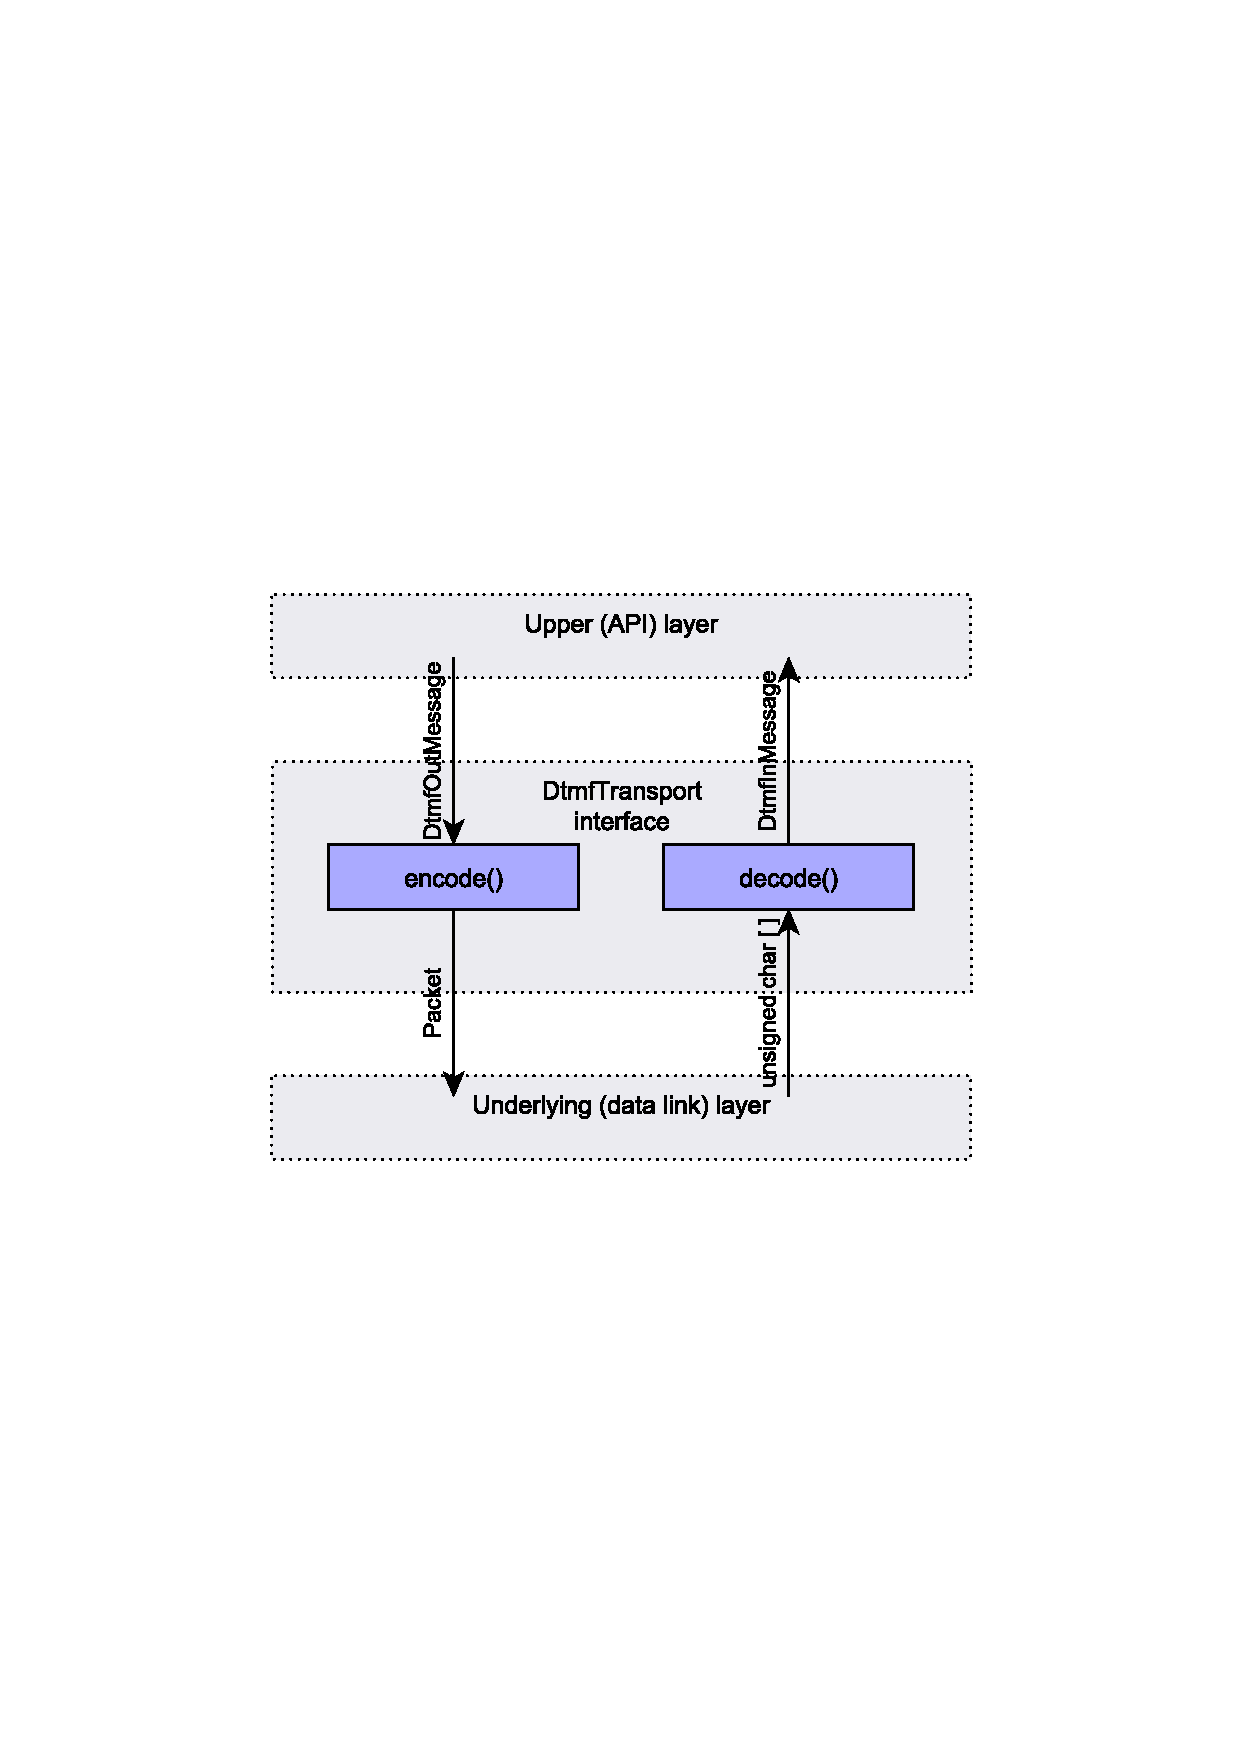
\includegraphics[scale=0.66,trim=0 280 0 275]{content/graphics/transport/trans_encode_decode.pdf}%trim=l b r t
 \caption{The transport layer protocol main interface methods}
 \label{fig:trans_encode_decode}
\end{figure}

Figure \ref{fig:trans_encode_decode} shows the \custtt{encode()} and \custtt{decode()} functions, and what they expect of in- and output from the above API and the underlying data link layer.

%setPort
%connect

\subsection{Encoding messages from the API}
To first gain overview of the \custtt{encode()} method, we see that it requires a message in the form of a \custtt{DtmfOutMessage} object, as described in more detail in Section \ref{sub:api_method_description}. This message object from the API contains the receivers port number as well as a pointer to an array of data. This is the data we want cut into pieces of the right size, to enclose in the \custtt{Packet} object.

What happens, when a suitable amount of data is ''cut'', is that \custtt{DtmfTransport} creates a new instance of the \custtt{Packet} object. All fields except for the receiver port number is filled out by \custtt{DtmfTransport} automatically without user interaction. This object then contains all of the information to pass on to the underlying layer.


\subsection{Decoding messages from the data link layer}
The method of choice, to pass data from the data link layer to the transport layer protocol, is chosen to simply be an array of bytes. These bytes are really stored in a buffer by the data link layer protocol. A pointer to this buffer is then passed on to the transport protocol. It is then the protocols responsibility to make sense of this array of bytes. This is done via the \custtt{packetFromCharBuffer()} method, which is a member of \custtt{DtmfTransport}. It examines the buffer to see if there is enough data to make out the header: If there is, a packet header will be assembled to then find out whether

%The \custtt{encode()} method is the method handling messages coming from the above layer (here: The API) 

%
%The packet is such a significant, and recurring, data structure that it is implemented as it's own class. It's most significant data members a
%
% 2 classes
% functions typer: compability/functionality
%
%
%
%
%
%
%
%